\PassOptionsToPackage{unicode=true}{hyperref} % options for packages loaded elsewhere
\PassOptionsToPackage{hyphens}{url}
%
\documentclass[]{article}
\usepackage{lmodern}
\usepackage{amssymb,amsmath}
\usepackage{ifxetex,ifluatex}
\usepackage{fixltx2e} % provides \textsubscript
\ifnum 0\ifxetex 1\fi\ifluatex 1\fi=0 % if pdftex
  \usepackage[T1]{fontenc}
  \usepackage[utf8]{inputenc}
  \usepackage{textcomp} % provides euro and other symbols
\else % if luatex or xelatex
  \usepackage{unicode-math}
  \defaultfontfeatures{Ligatures=TeX,Scale=MatchLowercase}
\fi
% use upquote if available, for straight quotes in verbatim environments
\IfFileExists{upquote.sty}{\usepackage{upquote}}{}
% use microtype if available
\IfFileExists{microtype.sty}{%
\usepackage[]{microtype}
\UseMicrotypeSet[protrusion]{basicmath} % disable protrusion for tt fonts
}{}
\IfFileExists{parskip.sty}{%
\usepackage{parskip}
}{% else
\setlength{\parindent}{0pt}
\setlength{\parskip}{6pt plus 2pt minus 1pt}
}
\usepackage{hyperref}
\hypersetup{
            pdftitle={Mobilite\_RATP},
            pdfauthor={Selim Ach},
            pdfborder={0 0 0},
            breaklinks=true}
\urlstyle{same}  % don't use monospace font for urls
\usepackage[margin=1in]{geometry}
\usepackage{graphicx,grffile}
\makeatletter
\def\maxwidth{\ifdim\Gin@nat@width>\linewidth\linewidth\else\Gin@nat@width\fi}
\def\maxheight{\ifdim\Gin@nat@height>\textheight\textheight\else\Gin@nat@height\fi}
\makeatother
% Scale images if necessary, so that they will not overflow the page
% margins by default, and it is still possible to overwrite the defaults
% using explicit options in \includegraphics[width, height, ...]{}
\setkeys{Gin}{width=\maxwidth,height=\maxheight,keepaspectratio}
\setlength{\emergencystretch}{3em}  % prevent overfull lines
\providecommand{\tightlist}{%
  \setlength{\itemsep}{0pt}\setlength{\parskip}{0pt}}
\setcounter{secnumdepth}{0}
% Redefines (sub)paragraphs to behave more like sections
\ifx\paragraph\undefined\else
\let\oldparagraph\paragraph
\renewcommand{\paragraph}[1]{\oldparagraph{#1}\mbox{}}
\fi
\ifx\subparagraph\undefined\else
\let\oldsubparagraph\subparagraph
\renewcommand{\subparagraph}[1]{\oldsubparagraph{#1}\mbox{}}
\fi

% set default figure placement to htbp
\makeatletter
\def\fps@figure{htbp}
\makeatother

\usepackage{booktabs}
\usepackage{longtable}
\usepackage{array}
\usepackage{multirow}
\usepackage{wrapfig}
\usepackage{float}
\usepackage{colortbl}
\usepackage{pdflscape}
\usepackage{tabu}
\usepackage{threeparttable}
\usepackage{threeparttablex}
\usepackage[normalem]{ulem}
\usepackage{makecell}
\usepackage{xcolor}

\title{Mobilite\_RATP}
\author{Selim Ach}
\date{18/10/2020}

\begin{document}
\maketitle

Ce document est rédigé à des fins d'illustration et l'analyse se base
sur des données publiques provenant de la RATP. L'analyse statistique
est faite avec le logiciel de programmation R, et a pour but de donner
un aperçu des différentes possibilités de traitement de données, de
production d'indicateurs et autres graphiques.

\begin{center}\rule{0.5\linewidth}{0.5pt}\end{center}

Source - \url{https://dataratp2.opendatasoft.com/explore/?sort=modified}

Ce jeu de données détaille le trafic des entrants directs sur le réseau
ferré RATP en 2019.

Les « entrants directs » sont exclusivement les voyageurs provenant de
la voie publique ou du réseau SNCF entrant sur le réseau de transport
RATP en validant un titre de transport valide.

Les voyageurs en correspondance (y compris correspondances métro/RER)
sur le réseau RATP ne sont pas comptabilisés.

\hypertarget{statistiques-descriptives-guxe9nuxe9rales}{%
\subsubsection{Statistiques descriptives
générales}\label{statistiques-descriptives-guxe9nuxe9rales}}

\hypertarget{fruxe9quentation}{%
\paragraph{Fréquentation}\label{fruxe9quentation}}

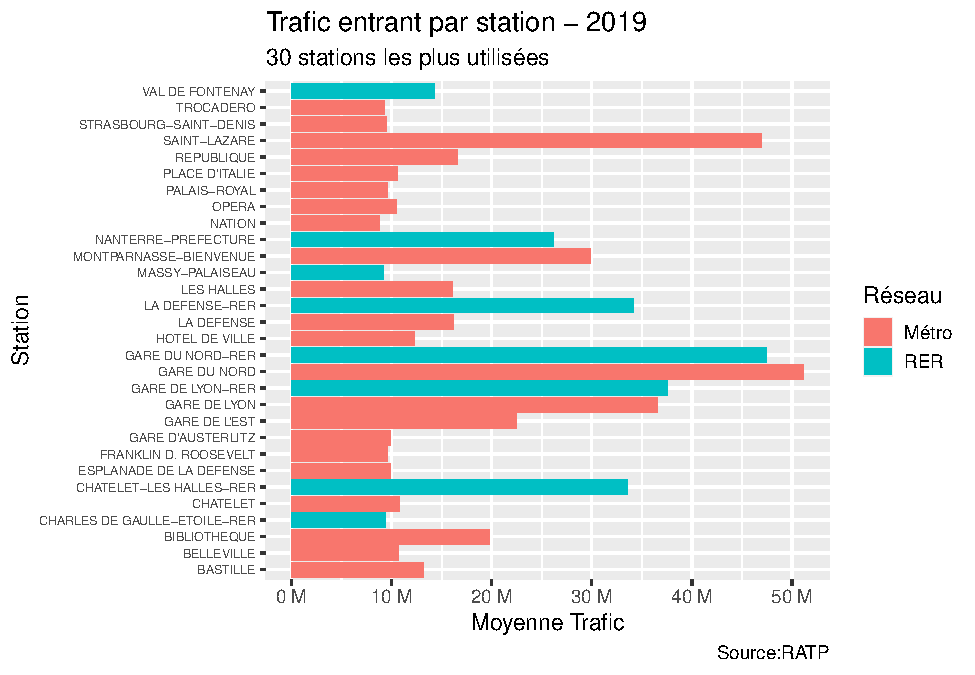
\includegraphics{Mobilite_RATP_files/figure-latex/unnamed-chunk-2-1.pdf}

\hypertarget{moyenne-fruxe9quentation-maximale-et-minimale}{%
\paragraph{Moyenne, fréquentation maximale et
minimale}\label{moyenne-fruxe9quentation-maximale-et-minimale}}

\begin{table}[H]
\centering
\begin{tabular}{l|r|r|r}
\hline
Réseau & Moyenne & Max & Min\\
\hline
Métro & 4,593,587 & 51,141,374 & 169,939\\
\hline
RER & 6,046,202 & 47,417,703 & 419,294\\
\hline
\end{tabular}
\end{table}

\hypertarget{statistiques-descriptives-par-ligne-de-muxe9tro-et-rer}{%
\subsubsection{Statistiques descriptives par ligne de métro et
RER}\label{statistiques-descriptives-par-ligne-de-muxe9tro-et-rer}}

\hypertarget{pic-voyageurs---rer}{%
\paragraph{Pic voyageurs - RER}\label{pic-voyageurs---rer}}

\begin{table}[H]
\centering
\begin{tabular}{l|l|r}
\hline
Réseau & Station & Trafic\\
\hline
RER & GARE DU NORD-RER & 47,417,703\\
\hline
\end{tabular}
\end{table}

\hypertarget{pic-voyageurs---muxe9tro}{%
\paragraph{Pic voyageurs - Métro}\label{pic-voyageurs---muxe9tro}}

\begin{table}[H]
\centering
\begin{tabular}{l|l|r}
\hline
Réseau & Station & Trafic\\
\hline
Métro & GARE DU NORD & 51,141,374\\
\hline
\end{tabular}
\end{table}

\hypertarget{ruxe9partition-des-voyageurs-rer-et-muxe9tro}{%
\subsubsection{Répartition des voyageurs RER et
Métro}\label{ruxe9partition-des-voyageurs-rer-et-muxe9tro}}

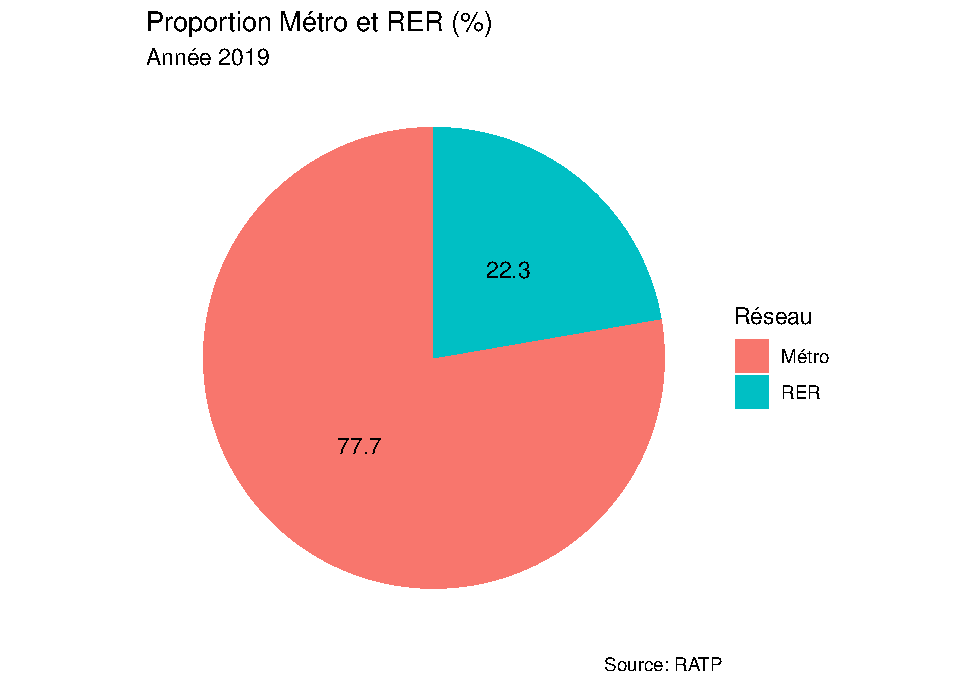
\includegraphics{Mobilite_RATP_files/figure-latex/unnamed-chunk-7-1.pdf}

\hypertarget{ruxe9partition-des-voyageurs-sur-les-lignes-principales-et-par-ville-hors-paris}{%
\subsubsection{Répartition des voyageurs sur les lignes principales et
par ville (hors
Paris)}\label{ruxe9partition-des-voyageurs-sur-les-lignes-principales-et-par-ville-hors-paris}}

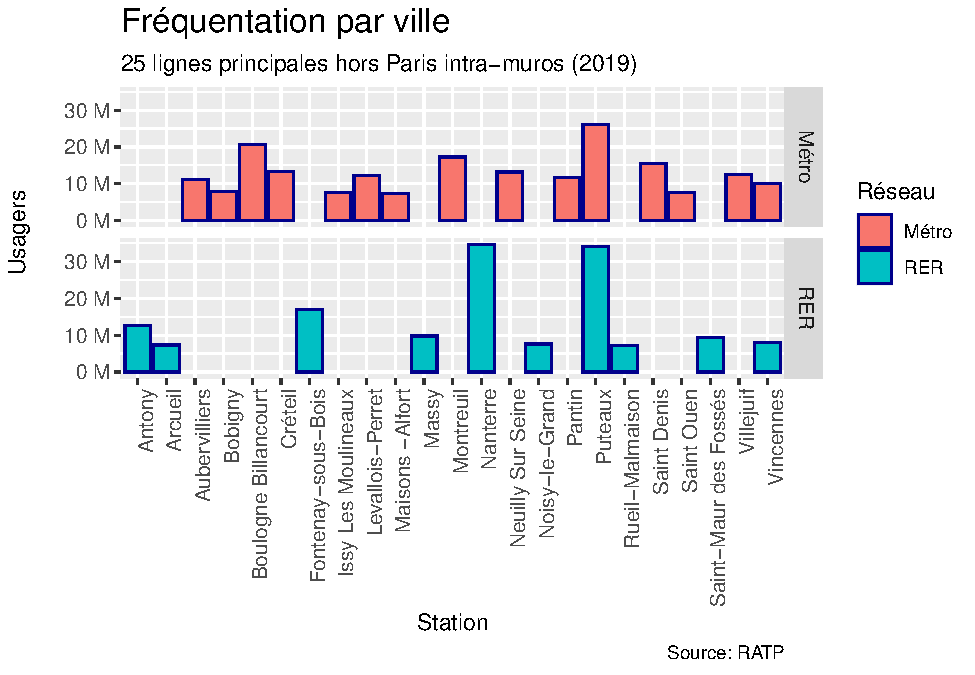
\includegraphics{Mobilite_RATP_files/figure-latex/unnamed-chunk-9-1.pdf}

\end{document}
